% CREATED BY DAVID FRISK, 2018
\chapter{Marco teórico}

Un marco conceptual es una herramienta analítica con variaciones y contextos. Se puede aplicar en diferentes categorías de trabajo donde se necesita una imagen general. Se usa para hacer distinciones conceptuales y organizar ideas.

\section{Ejemplos}
En esta sección se muestran algunos ejemplos de la utilización de latex.
    \subsection{Figura}
    En esta subsección se muestra como se realiza una referencia cruzada a una imagen, por ejemplo la de la figura \ref{grafica}.
    
    \begin{figure}[H]
    \centering
    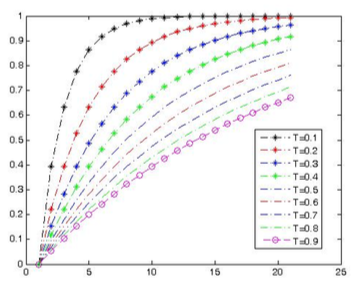
\includegraphics[scale=0.5]{include/2_MTeorico/Figures/primOrden.png}
    \caption{Modelo de primer orden para diferentes constantes de tiempo.}
    \label{grafica}
    \end{figure}

    \subsection{Ecuaciónes}
    En esta subsección se muestra el uso de ecuaciones con latex, como la de la ecuación \ref{ecuacionej}.
    \begin{equation}
    \min_{u} f_{objetivo} = \sum_{i}(y_{i}- \hat y_{i})^{2}
    \label{ecuacionej}
    \end{equation}

    \subsection{Tablas}
    En esta subsección se muestra el uso de tablas con latex, como la de la tabla \ref{tablaEj}.
    \begin{table}[H]
    \centering
    \caption{Valores de $f(t)$ para $t=0,1,\dots 5$.}
    \begin{tabular}{l|llllll} \hline\hline
    $t$ & 0 & 1 & 2 & 3 & 4 & 5 \\ \hline
    $f(t)$ & 1 & 1 & 4 & 9 & 16 & 25 \\ \hline\hline
    \end{tabular}
    \label{tablaEj}
    \end{table}

    \subsection{Listas}
     En esta subsección se muestra el uso de Listas con latex, como la que se muestra a continuación.
    \begin{enumerate}
    \item Primera
    \begin{enumerate}
        \item Sub primero
        \item Sub Segundo
    \end{enumerate}
    \item Segunda
    \item Tercera 
    \item \dots
    \end{enumerate}

    \subsection{Lista de codigo fuente}
    En esta subsección se muestra el uso listas de códigos de programación con latex, como el que se muestra a continuación.
    \begin{lstlisting}
    #include <stdio.h>
    int main()
    {
        int i;
        for (i = 0; i < 10; i++)
        {
        printf("Hello world!");
        }
    return 0;
    }
    \end{lstlisting}

    \subsection{Recursos}
    Codecogs, un minieditor para compartir los resultados hasta como imagen.
    \begin{figure}[H]
    \centering
    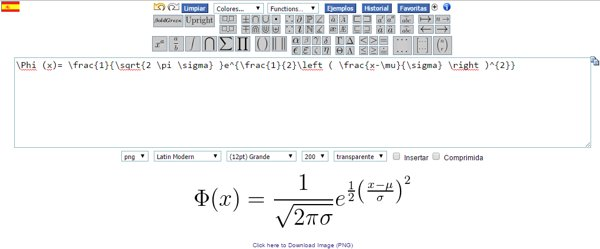
\includegraphics[scale=0.8]{include/2_MTeorico/Figures/codecogs.jpg}
    \caption{Captura minieditor de ecuaciones en linea Codecogs.}
    \end{figure}
    Con LaTeX Table Generador se puede hacer todo lo anterior visualmente partiendo de unos datos importados tanto de un archivo de texto como desde hojas de cálculo (copiando y pegando).
    \begin{figure}[H]
    \centering
    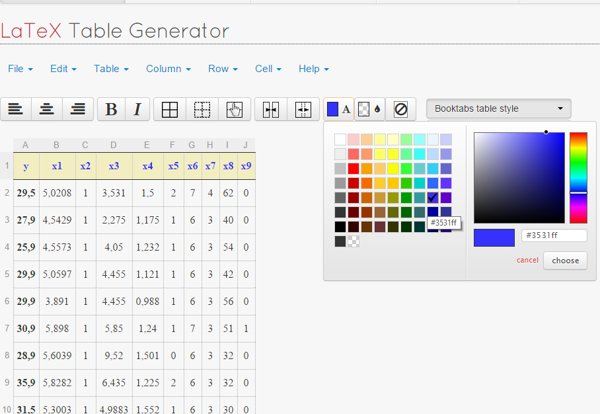
\includegraphics[scale=0.8]{include/2_MTeorico/Figures/latex-table-generator.jpg}
    \caption{Captura de la herramienta LaTeX Table Generator. }
    \end{figure}
    
    \subsection{Uso y ejemplo de secciones}
    En la tabla \ref{tablaSec} se muestra el uso de los niveles de las secciones.
    \begin{table}[H]
   
    \centering
    \caption{Uso de las secciones en el documento.}
    \begin{tabular}{ll} \hline\hline
    Name & Command\\ \hline
    Chapter & \textbackslash\texttt{chapter\{\emph{Chapter name}\}}\\
    Section & \textbackslash\texttt{section\{\emph{Section name}\}}\\
    Subsection & \textbackslash\texttt{subsection\{\emph{Subsection name}\}}\\
    Subsubsection & \textbackslash\texttt{subsubsection\{\emph{Subsubsection name}\}}\\
    Paragraph & \textbackslash\texttt{paragraph\{\emph{Paragraph name}\}}\\
    Subparagraph & \textbackslash\texttt{paragraph\{\emph{Subparagraph name}\}}\\ \hline\hline
    \end{tabular}
    \label{tablaSec}
    \end{table}
    
    

    \subsection{Nomenclatura}
    Aquí se incluye una nomencladura.
    \nomenclature{$\mathbb{R}$}{Real Numbers}
    \nomenclature{$\mathbb{C}$}{Complex Numbers}
    \nomenclature{$\mathbb{H}$}{Quaternions}
    
     \subsection{Citas}
    Este es un ejemplo de una cita \cite{NAKASUKA2004919}.
    \cite{einstein}.



